% !TEX encoding = UTF-8 Unicode
\documentclass[fr]{../../../eplsummary}
\usepackage{setspace}
\usepackage{framed}
\usepackage{pgfplots}

\hypertitle[']{Analyse}{1}{EPL}{1102}{Philippe Dan}{Jean-François Remacle et François Glineur}

%Header

\newpage

\tableofcontents

\section{Suites et séries}
Une suite est une liste ordonnée de nombres. L'index d'un terme est toujours un nombre entier. Notation : $\{a_n\}$ désigne une suite.
\paragraph{Suite par récurrence} Une suite est définie par récurrence lorsque chaque terme est calculé à partir du précédent.
\paragraph{Suite explicite} Une suite est explicite lorsque chaque terme est calculé à partir de son index.
\subsection{Convergence}
Une suite converge si :
\begin{equation}
    \quad \exists N : \forall n > N : |a_n - a| < \epsilon
\end{equation}
\subsubsection{Suite de Héron}
\begin{equation}
    a_{n+1} = \frac{1}{2}\left(a_n + \frac{2}{a_n}\right)
\end{equation}
Si l'on remplace le 2 par un autre nombre, alors la suite converge vers la racine de ce nombre.
\subsubsection{Démonstration de la convergence}
Pour démontrer qu'une suite est convergente, considérons : $a_n = \frac{n+3}{n+2}$. Les termes de cette suite tendent vers la valeur de 1. Donc on a ainsi $a = 1$. À présent, vérifions si le postulat est vrai :
\begin{gather}
    \left| \frac{n+3}{n+2} - 1\right| < \epsilon \quad \text{?} \\
    \left| \frac{1}{n+2}\right| < \epsilon \quad \text{On met sur le même dénominateur} \\
    \frac{1}{n+2} < \epsilon \Rightarrow n + 2 > \frac{1}{\epsilon} \quad \text{On prend l'inverse} \\
    n > \frac{1}{\epsilon} - 2 \Rightarrow n > \frac{1}{\epsilon} \quad \text{Que l'on prenne $\frac{1}{\epsilon}$ ou $\frac{1}{\epsilon} - 2$, cela revient au même} \\
    \text{Ainsi, si on pose n = $\epsilon + 1$, le postulat est toujours vrai. La suite converge} \\
\end{gather}
\begin{flushright}
    $\square$
\end{flushright}
\subsubsection{Théorème 1.6}
Soit ${a_n}$ et ${b_n}$ deux suites convergentes. On a :
\begin{equation}
    \lim_{n\rightarrow \infty} a_n = a \quad \lim_{n\rightarrow \infty} b_n = b
\end{equation}
\paragraph{Propriétés}
\begin{gather}
    \lim_{n\rightarrow \infty} (a_n+b_n) = a+b \\
    \lim_{n\rightarrow \infty} (a_n\cdot b_n) = a\cdot b \\
    \text{Si $a\ne 0$}, \lim_{n\rightarrow \infty} \frac{1}{a_n} = \frac{1}{a}
\end{gather}
\subsubsection{Théorème du sandwich}
Supposons que pour $n > N$ on a :
\begin{equation}
    a_n \leq b_n \leq c_n \Rightarrow a_n-a \leq b_n - a \leq c_n - a
\end{equation}
Si $a_n$ et $c_n$ ont la même limite et si elles convergent, alors:
\begin{gather}
    \exists N_1 : \forall n > N_1 : \left|a_n - a \right| < \epsilon \\
    \exists N_2 : \forall n > N_2 : \left|c_n - a \right| < \epsilon \nonumber
\end{gather}
Ainsi, en prenant $N=max(N_1,N_2)$ on a que $b_n$ est "piégée" entre deux suites qui convergent, et donc elle converge elle aussi nécessairement.
\subsubsection{Théorème 1.8 : Toute suite convergente est bornée.}
C'est-à-dire que ${a_n}$ est bornée si $a_n \in [-B;B]$. Prouvons-le. Considérons ${a_n}$ une suite convergente vers $a$. Alors,
\begin{gather}
    \exists N : \forall n > N : \left| a_n -a \right| < 1 \\
    \text{On sait que :} \quad |a_n| = |a + a_n - a| \\
    \text{Par l'inégalité triangulaire, on a :} \quad |a + a_n -a| \leq |a| + |a_n-a| \leq |a| + 1 \\
    \text{Ainsi, $|a_n| \leq |a| + 1$ prouve que la suite est bornée.} \nonumber
\end{gather}
\begin{flushright}
    $\square$
\end{flushright}
\subsubsection{Théorème 1.9 : Une suite bornée converge}
\subsubsection{Théorème 1.10 : Une suite monotone bornée converge}
\subsection{Suites géométriques}
Une suite géométrique est une suite où chaque terme est égal au précédent multiplié par une raison r. ($r \in \mathbb{R} $) \\ Une suite géométrique est notée : $\{r^n\}$
\subsubsection{Théorème 1.11}
Une suite géométrique converge ou diverge. 
\begin{gather}
    \text{Si} \quad |r| < 1 \Rightarrow \lim_{n\rightarrow \infty} r^n = 0 \\
    \text{Si} \quad |r| = 1 \Rightarrow \lim_{n\rightarrow \infty} 1^n = 1 \\
    \text{Si} \quad |r| > 1 \Rightarrow \text{Diverge} \nonumber
\end{gather}
Prenons à présent la suite $\{(-1)^{n}\}$. Montrons qu'elle ne converge pas.
\begin{gather}
    \text{Si nous prenons} \quad \epsilon = \frac{1}{2}, a=0 \Rightarrow |a_n - 0| = 1 \nless \epsilon 
\end{gather}
\begin{flushright}
    $\square$
\end{flushright}
Essayons maintenant de trouver la convergence de la suite $a_n = \left(\frac{n!}{n^n}\right)^{\frac{1}{n}}$. Pour savoir si cette suite est décroissante ou croissante, passons au $ln$ de cette suite. 
\begin{framed}
En effet, si la composée d'une fonction est décroissante alors les deux fonctions ont une croissance opposée, si elle est croissante alors elles ont la même croissance.
\end{framed}
\begin{gather}
    \ln{a_n} = \frac{1}{n} \cdot \underbrace{\ln{\left( \frac{n!}{n^n} \right)} }_{décroissante} \quad \text{Donc, comme $\ln$ est croissante, $a_n$ est décroissante.} \\
    \ln{a_n} = \frac{1}{n} \cdot \ln{\left(\frac{n(n-1)(n-2)...1}{n\cdot n\cdot n...\cdot n}\right)} = \frac{1}{n} \cdot \sum_{k=1}^n \ln{\left(\frac{k}{n}\right)} \\ \text{En effectuant la limite vers l'infini, on tombe sur la définition de l'intégrale de Riemann} \\
    \lim_{n\rightarrow +\infty}{\ln{a_n}} = \int_0^1 \ln{x}\,dx = -1 \quad \text{Car $0 < \ln a_n \leq 1$}\\
    \text{Et donc, } \quad \lim_{n\rightarrow +\infty} a_n = \frac{1}{e}
\end{gather}
\begin{flushright}
    $\square$
\end{flushright}

\begin{figure}[h]
    \centering
    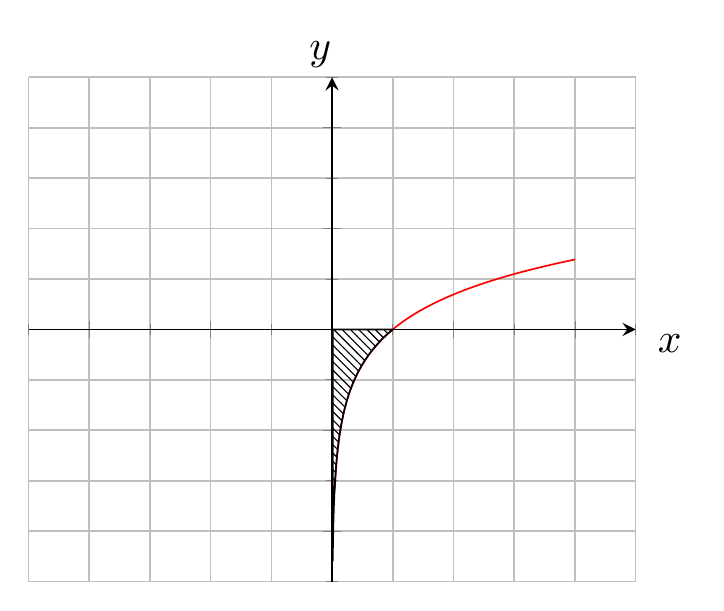
\begin{tikzpicture}[scale=1.5]
        \usetikzlibrary{patterns}
        \begin{axis}[grid=both,ymin=-5,ymax=5,xmax=5,xmin=-5,xticklabel=\empty,yticklabel=\empty,
               minor tick num=1,axis lines = middle,xlabel=$x$,ylabel=$y$,label style =
               {at={(ticklabel cs:1.1)}},scale=0.75]
        \addplot[color=red,domain=0:4,samples=100] {ln(x)};
        \addplot[pattern=north west lines, domain=0:1,samples=100] {ln(x)} \closedcycle;
        \end{axis}
    \end{tikzpicture}
    \caption{Illustration}
    \label{fig:my_label}
\end{figure}

    
\subsection{Séries de Taylor}
Si on part d'une suite $\{a_n\}$, la série $s_n$ est définie comme une suite dont chaque terme $s_n$ est une somme partielle des $n$ éléments de la suite $a_n$.
\begin{equation}
    s_n = \sum_{i=1}^n a_n
\end{equation}
Cette série converge sous les mêmes conditions qu'une suite classique.
\subsubsection{Théorème 1.12}
\begin{gather}
    \text{Si} \, \sum_{n=1}^{\infty} a_n \,\text{converge, alors }\lim_{+\infty} a_n = 0
\end{gather}
\subsubsection{Théorème 1.13}
\begin{equation}
    \text{Si}\, |x|<1 \, \text{alors} \, S_n = 1+x+x^2+x^3+...+x^n \,\text{converge et} \, \lim_{n\rightarrow +\infty} s_n = \sum_0^\infty x^n = \frac{1}{1-x}
\end{equation}
Démonstration en considérant $s_n\cdot (1-x)$ :
\begin{gather}
    \begin{array}{rl}
        s_n\cdot (1-x) = &(1+x+x^2+x^3+...+x^n)\cdot(1-x) 
        \\ = &(1+x+x^2+...+x^n)-(x+x^2+...+x^n+x^{n+1}) = 1-x^{n+1} \\
    \end{array} \\ 
    \text{Donc} \quad s_n = \frac{1-x^{n+1}}{1-x} \Rightarrow \lim_{n\rightarrow +\infty}\frac{1-x^{n+1}}{1-x} = \frac{1}{1-x}
\end{gather}
\begin{center}
    Si $|x|\geq 1$ la suite diverge.
\end{center}
\subsubsection{Théorème 1.14 : Comparaison}
\begin{gather}
    \text{Supposons les suites} \quad 0\leq a_n \leq b_n \\ 
    \text{Alors si la série} \, \sum_{1}^{\infty}b_n \quad \text{converge, alors} \, \sum_{1}^{\infty}a_n \, \text{converge aussi.}
\end{gather}
\subsubsection{Théorème 1.15 : Comparaison des limites}
\begin{gather}
    \text{Supposons les suites $a_n$ et $b_n$} \\ 
    \text{Alors si} \, \lim_{n\rightarrow +\infty}\frac{a_n}{b_n} \in \mathbb{R}^+ \Rightarrow \sum_{1}^{\infty}a_n \, \text{converge, si} \, \sum_{1}^{\infty}b_n \, \text{converge aussi.}
\end{gather}
\subsubsection{Théorème 1.16}
\begin{gather}
    \text{Si} \quad \sum_{1}^{\infty}|a_n| \, \text{converge, alors} \, \sum_{1}^{\infty}a_n \, \text{converge aussi.}
\end{gather}
Attention, la réciproque n'est pas vraie.
\paragraph{Exemple d'utilisation}
\begin{gather}
    \text{Soit} \quad \sum_{n=1}^{\infty}\frac{1}{(-2)^n\cdot n} \quad \text{Calculons} \quad \sum_{n=1}^{\infty}\left|\frac{1}{(-2)^n\cdot n}\right| = \sum_{n=1}^{\infty}\frac{1}{2^n\cdot n} \\
    \text{Or, comme} \quad \sum_{n=1}^{\infty}\left(\frac{1}{2}\right)^n \quad \text{converge (théorème 1.13)} \\
    \text{Et comme } \quad 0\leq \sum_{n=1}^{\infty}\frac{1}{(2)^n\cdot n} \leq \sum_{n=1}^{\infty}\left(\frac{1}{2}\right)^n \quad \text{la série initiale converge.}
\end{gather}
Prenons une autre suite à présent.
\begin{gather}
    \text{Soit} \quad \sum_{n=1}^{\infty}\frac{(-1)^{n-1}}{n} \\
    \text{Prenons les termes pairs} \quad S_{2k} = \underbrace{1 - \frac{1}{2}}_{<\,0} + \underbrace{\frac{1}{3} - \frac{1}{4}}_{<\,0}... - \frac{1}{2k} \quad \text{La série est donc croissante} \\
    \text{De plus, elle est bornée par 1 car on ajoute à chaque fois une somme $< 0,5$ au terme de base $0,5$. } \\ 
    \text{Raisonnement identique pour les termes impairs (décroissant, bornée par $0,5$ par le bas)} \\
    \text{En calculant les limites respectives et en les soustrayant, on obtient 0, la limite de la série.}\\ 
    \text{La série est donc bien convergente. (th. 1.10)}
\end{gather}
\begin{flushright}
    $\square$
\end{flushright}
\subsubsection{Théorème 1.7}
Soit une suite décroissante bornée par 0.
\begin{gather}
    \text{Si} \quad \lim_{\infty}a_n = 0 \Rightarrow \sum_{n=1}^{\infty} (-1)^n a_n \quad \text{converge.}
\end{gather}
\subsubsection{Définition 1.7}
\begin{gather}
    \text{Si} \quad \sum_{i=1}^{\infty} a_i \: \text{converge, et si } \: \sum_{i=1}^{\infty} |a_i| \: \text{converge, alors la série "converge absolument".} \\
    \text{Si} \quad \sum_{i=1}^{\infty} a_i \: \text{converge, et si } \: \sum_{i=1}^{\infty} |a_i| \: \text{diverge, alors la série "converge partiellement" ou "sous condition".} \\
\end{gather}
\subsubsection{Ratio test}
Supposons deux termes d'une suite : $a_{n+1}$ et $a_n$. Prenons la limite de leur quotient en valeur absolue.
\begin{gather}
    \text{Si} \: \lim_{n\rightarrow \infty} \left| \frac{a_{n+1}}{a_n} \right| = L < 1 \Rightarrow \sum_{i=1}^{\infty} a_n \quad \text{converge absolument.} \\
    \text{Si} \: \lim_{n\rightarrow \infty} \left| \frac{a_{n+1}}{a_n} \right| = L > 1 \Rightarrow \sum_{i=1}^{\infty} a_n \quad \text{diverge.} \\
    \text{Dans le cas L = 1, on n'a aucune information.}
\end{gather}
\subsection{Suites de Cauchy}
Une suite de cauchy $a_n$ est définie comme ceci :
\begin{equation}
    \forall \epsilon \: \exists N : \forall m,n > N : |a_m - a_n| < \epsilon
\end{equation}
\subsubsection{Théorème 1.20}
Toute suite de Cauchy converge dans $\mathbb{R}$. Réciproquement, toute suite qui converge est une suite de Cauchy.
\paragraph{Exemple}
Montrons que la série harmonique $S_n = \sum \frac{1}{i}$ n'est pas une suite de Cauchy.
\begin{gather}
    S_n = \sum_{i=1}^n \frac{1}{i} \quad S_{2n} = \sum_{i=1}^{2n} \frac{1}{i} \\
    S_{2n} - S_n = \sum_{i=n+1}^{2n}\frac{1}{i} \text{Car il ne nous reste plus que les éléments après n.} \\
    \sum_{i=1}^{n}\frac{1}{i} \geq \sum_{i=1}^{2n} \frac{1}{i} \Rightarrow \frac{1}{n} \geq \frac{1}{2n} \Rightarrow 1 > \frac{1}{2} \\
    \text{Différence toujours plus grande que $\frac{1}{2}$, la série ne converge pas.}
\end{gather}
\begin{flushright}
    $\square$
\end{flushright}
\subsection{Le nombre e}
Il est défini comme suit :
\begin{gather}
    e = \lim_{n\rightarrow \infty} \left(1 + \frac{1}{n} \right)^{n}
\end{gather}
Cette définition converge très lentement vers e. D'autres techniques existent pour obtenir la valeur de e plus rapidement.
\section{Fonctions et continuité}
\subsection{Notion de fonction}
Voir livre.
\subsection{Continuité}
\begin{framed}
Une fonction est continue lorsque : 
\begin{equation}
    \forall \epsilon > 0, \exists \delta > 0, \forall x,a \in dom f(x)\quad  : \quad |x-a| < \delta \Rightarrow |f(x) - f(a)| < \epsilon
\end{equation}
\end{framed}
On dit d'une fonction qu'elle est bornée lorsqu'il existe un réel B tel que $-B \leq f(x) \leq B$. Par exemple la fonction $f(x) = \frac{1}{x^2+1}$ est bornée par $B = 1$.
\newline \indent Si une fonction est toujours supérieur à un réel $B > 0$ alors on dit qu'elle s'éloigne de 0. La fonction ci-dessus ne s'éloigne pas de zéro.
\subsubsection{Notion de limite}
On dit que :
\begin{gather}
    \lim_{x\rightarrow c} f(x) = L \Longleftrightarrow \forall \epsilon,\exists \delta : |x-c| < \delta \Rightarrow |f(x) - L| < \epsilon
\end{gather}
La fonction f est alors continue si pour tout $x,c$ on a :
\begin{equation}
    \lim_{x\rightarrow c} f(x) = f(c)
\end{equation}
\subsubsection{Lien entre suite et fonction}
Si l'on considère une suite ${x_i}$ qui tend vers $c$, alors ${f(x_i)} \rightarrow L$.
Par exemple, on peut appliquer ce lien pour trouver la convergence de $n\sin{\frac{1}{n}}$.
\begin{gather}
    \lim_{x\rightarrow 0} \frac{\sin{x}}{x} = 1 \Rightarrow x_n = \frac{1}{n} \Rightarrow n\sin{\frac{1}{n}} = \frac{1}{x_n}\sin{x_n} = \frac{\sin{x_n}}{x_n} = 1
\end{gather}
\subsubsection{Continuité uniforme}
Une fonction est continue uniformément sur un intervalle s'il existe $\delta$ tel que la fonction soit continue sur tout l'interval (sans les extrémités).
\subsubsection{Théorème des valeurs intermédiaires}
\begin{framed}
Si une fonction est continue sur un intervalle $[a;b]$ alors la fonction prend toutes les valeurs entre $f(a)$ et $f(b)$.
\end{framed}
\subsubsection{Théorème de Roll}
\begin{framed}
Si une fonction est continue sur un intervalle $[a;b]$ alors la fonction possède au moins un minimum et un maximum sur cet intervalle.
\end{framed}
\subsubsection{Continuité de fonctions composées}
\begin{framed}
La composée de deux fonctions continues donne une fonction continue.
\end{framed}
\paragraph{Limite de fonctions composées}
\begin{equation}
    \lim_{x\rightarrow c} g(x) = L \Rightarrow \lim_{x\rightarrow c} (f \circ g)(x) = f(L) \Rightarrow \lim_{x\rightarrow c} f(g(x)) = f(\lim_{x\rightarrow c} g(x))z
\end{equation}
\subsubsection{Fonctions réciproques}
\begin{framed}
Si une fonction est strictement monotone et continue, alors la fonction réciproque de $f(x)$ existe et se note $f^{-1}(x)$
\end{framed}
\subsubsection{Fonction exponentielle}
La fonction exponentielle croit plus vite que la fonction polynôme. Aka, pour $k,n \in \mathbb{R} : k > 1$
\begin{gather}
    \lim_{x\rightarrow \infty} k^x\cdot x^n = +\infty
\end{gather}
\subsection{Suite et séries de fonctions}
\subsubsection{Convergence ponctuelle}
Soit une suite de fonction ${f_n}$ avec le même domaine. On dit que $f_n$ tend vers une fonction $f$ simplement (ponctuellement) si $\forall x: {f_n(x) \rightarrow f(x)}$.
Dans la plupart des cas, la convergence ponctuelle n'est pas intéressante. Si l'on prend cet exemple :
\begin{gather}
    x^n = g_n : [0;1] \Rightarrow g_n \rightarrow g(x) := \begin{cases}0\quad \forall x \in [0;1[ \\ 1 \quad \text{si} \, x= 1 \end{cases}
\end{gather}
On a une fonction qui n'est pas très intéressante.
\subsubsection{Convergence uniforme}
Si l'on considère un intervalle limité, alors si :
\begin{equation}
    \exists N : \forall n > N : |f_n(x) - f(x)| < \epsilon 
\end{equation}
Alors, $f_n$ converge uniformément vers $f(x)$.
\subsubsection{Propriétés}
Si l'on considère deux fonctions $f_n,g_n$ deux suites convergentes uniformément de fonctions continues sur $[a;b]$, alors:
\begin{itemize}
    \item $f_n+g_n$ converge uniformément vers $f+g$
    \item $f_n\cdot g_n$ converge uniformément vers $fg$
    \item Si $f\neq 0$ sur $[a;b]$, alors $\frac{1}{f_n}$ tend vers $\frac{1}{f}$ uniformément
    \item Si $h$ est une fonction continue sur $[a;b]$ alors $g_n \circ h$ converge uniformément vers $g\circ h$
    \item Si k est une fonction continue sur l'ensemble image de $g_n$ et $g$, alors $k \circ g_n$ converge uniformément vers $k\circ g$
\end{itemize}
\subsubsection{Séries de fonctions}
\paragraph{Séries entières}
Une série entière est une série de fonctions de la forme :
\begin{gather}
    \sum_{k=0}^{\infty} a_k(x-a)^k
\end{gather}
Les nombres $a_n$ sont appelés coefficients. Le nombre $a$ est appelé le centre de la série.
\paragraph{Propriétés}
Pour toute série entière un des cas suivants est toujours vrai.
\begin{enumerate}
    \item La série converge absolument pour chaque $x$
    \item La série converge seulement pour $x=a$
    \item Il existe un nombre positif $R$, appelé le rayon de convergence, tel que la série converge absolument pour $|x-a|<R$ et diverge pour $|x-a|>R$. Dans ce cas, il faut faire du cas par cas pour $x = a-R$ et $x=a+R$.
\end{enumerate}
\paragraph{Convergence uniforme d'une série entière}
Une série entière converge uniformément vers sa limite, sur n'importe quel intervalle $|x-a| < r$ où $r < R$. En particulier, la fonction limite est continue sur $[a-R;a+R]$.
\subsection{Dérivées}
La notion de dérivée permet de mettre en place l'approximation linéaire.
\subsubsection{Equations différentielles}
\paragraph{$y' = ky$}
Si l'on prend la forme $y' = ky$, alors les solutions sont $y = ce^{kx}$. Preuve :
\begin{gather}
    \text{Soit y une solution.} \quad \frac{y}{e^x} \Rightarrow \left(\frac{y}{e^x}\right)' = y'e^{-x} + y(-e)^{-x} = e^{-x}(y'-y) \\
    \text{Or, comme y' = y, car k = 1, on a : } \quad \left(\frac{y}{e^x}\right)' = 0 \Rightarrow \text{dérivée d'une constante}
\end{gather}
\paragraph{y'' = -y}
Les solutions de ce système sont de la forme : $a\cos x + b\sin x$. Preuve :
\begin{gather}
    \text{Cherchons $y:y'' = -y$, $y(0) = 0$, $y'(0) = 0$} \Rightarrow y = 0 \\
    \text{Posons $y_1,y_2$ des solutions quelconques. Si :} \quad \begin{cases}
        y_1(0) = y_2(0) \\
        y_1'(0) = y_2'(0)
    \end{cases} \Rightarrow y_1 = y_2 \\
    \text{Alors, } \quad y_1 '' - y_2'' = -(y_1-y_2) \\
\end{gather}
\section{Approximations de Taylor}
Grâce au théorème de Bolzano (valeurs intermédiaires), on en arrive au théorème des accroissements finis :
\begin{framed}
    Si f est continue et dérivable sur $]a;b[$ alors :
    \begin{gather}
        \exists c \in ]a;b[ : f'(c) = \frac{f(b)-f(a)}{b-a} = \text{pente de la sécante}
    \end{gather}
    Ce théorème est valable de manière générale aussi entre fonctions. (théorème 4.3).
\end{framed}
Considérons à présent le Lemme 4.1 : Soit une fonction continue sur $(a;b)$ et atteint sont maximum ou minimum au point c. Si $f'(c)$ existe, alors $f'(c) = 0$.
\newline \indent Prenons à présent $l_a : f(a) + \frac{f(b)-f(a)}{b-a}(x-a)$, la sécante. Considérons la différence $d(x) = f(x) - l(x)$.
\begin{itemize}
    \item d(a) = d(b) = 0 car la sécante passe par les extrémités
    \item Si le maximum et le minimum de d sont sur les bords, alors $d=0 \Rightarrow f = l$.
    \item Sinon, par le lemme, on a $d' = f' - l' \Rightarrow d'(c) = f'(c) - \frac{f(b)-f(a)}{b-a} = 0$
\end{itemize}
\subsection{Corollaire 4.1}
Une fonction dont la dérivée est nulle sur un intervalle est une fonction constante sur cet intervalle.
\subsection{Corollaire 4.2}
\begin{itemize}
    \item Si $f' > 0$ sur un intervalle, alors f est strictement croissante sur cet intervalle
    \item Si $f' >= 0$ sur un intervalle, alors f est non décroissante sur cet intervalle
    \item Si $f' < 0$ sur un intervalle, alors f est strictement décroissante sur cet intervalle
    \item Si $f' <= 0$ sur un intervalle, alors f est non croissante sur cet intervalle
\end{itemize}
\subsection{Extrema globaux et locaux}
\subsection{Théorème 4.2}
Suppose that f is continuous on an interval containing c, and that f(x) is positive for x less than c, and negative for x greater than c. Then f reaches its maximum on the interval at c. A similar characterization holds for the minimum.
\subsection{Théorème 4.3}
Théorème des accroissements finis généralisé. Il existe un point c tel que :
\begin{gather}
    \frac{f'(c)}{g'(c)} = \frac{f(b)-f(a)}{g(b)-g(a)}
\end{gather}
\subsection{Théorème 4.4 : Règle de l'Hospital}
\begin{gather}
    \text{Soit : } \quad \lim_{x\rightarrow a} f(x) = 0 \quad \lim_{x\rightarrow a} g(x) = 0 \\
    \text{Si la limite de leur quotient existe, alors : } \quad \lim_{x\rightarrow a} \frac{f(x)}{g(x)} = \lim_{x\rightarrow a} \frac{f'(x)}{g'(x)}
\end{gather}
\subsection{Définition 4.2}
Une fonction est n fois dérivable si la n-1 ème dérivée est dérivable. On note ça :
\begin{equation}
    f^{(n)} = \frac{d^n f}{dx^n}
\end{equation}
\subsection{Définition 4.3}
Une fonction est dérivable continuellement sur un intervalle si sa dérivée existe et est continue sur cet intervalle. Et le raisonnement est identique pour n fois dérivable continuellement.
\subsection{Informations apportées par la dérivée seconde}
Considérons $m \leq f'' \leq M$ sur $[a;b]$. Prenons en compte la partie gauche de l'inéquation.
\begin{gather}
    M \geq f'' \Rightarrow M - f'' \geq 0 \Rightarrow \frac{d}{dx}[Mx - f'] \geq 0 \Rightarrow Mx-f' \geq Ma - f'(a) \\ \text{Ceci nous indique que $Mx-f'(x)$ est non décroissante. On peut réécrire :} \quad Mx - Ma \geq f'(x) - f'(a) \\
    M(x-a) \geq f'(x) - f'(a) \Rightarrow \frac{d}{dx}\left(M\frac{(x-a)^2}{2}\right) \geq \frac{d}{dx}\left[f(x)-xf'(a)\right] \\ \frac{d}{dx}\left(M\frac{(x-a)^2}{2}-\left[f(x)-xf'(a)\right]\right) \geq 0 \\
    \text{Ainsi, de même, on a que la primitive du terme de gauche est une fonction non décroissante.} \\
    M\frac{(x-a)^2}{2} + xf'(a) - f(x) \geq af'(a) - f(a) \\
    f(x) \leq f(a)+f'(a)(x-a)+M\frac{(x-a)^2}{2}
\end{gather}
En faisant le même processus sur le membre de gauche, on obtient une inégalité générale, qui n'est autre que l'inégalité de Taylor.
\subsubsection{Approximation linéaire théorème 4.5}
Si l'on prend une fonction f dérivable deux fois sur un intervalle $[a;b]$, alors $\exists c \in [a;b]$ tel que :
\begin{gather}
    f(b) = f(a) + f'(a)(b-a) + f''(c)\frac{(b-a)^2}{2}
\end{gather}
\subsection{Définition 4.4}
Une fonction dont le graphe est au-dessus de ses tangentes est une fonction convexe.
\subsection{Théorème 4.8}
Considérons une fonction f dérivable deux fois sur l'intervalle $[a;b]$, et $f'' > 0$. Alors, pour chaque $x \in (a;b)$, on a :
\begin{gather}
    f(x) < f(b)\frac{x-a}{b-a} + f(a)\frac{b-x}{b-a}
\end{gather}
Ce théorème dit que le graphe d'une fonction convexe se situe en-dessous de la sécante $[a;b]$.
\subsection{Théorème de Taylor}
Si l'on considère l'inégalité suivante d'une fonction n fois dérivable pour tout $x \in [a;b]$ : $ m \leq f^{(n)} \leq M$. Alors, on a : 
\begin{gather}
    f(a) + f'(a)(x-a) + f''(a)\frac{(x-a)^2}{2!}+...+f^{(n-1)}(a)\frac{(x-a)^{n-1}}{(n-1)!} + m\frac{(x-a)^n}{n!} \\
    \leq f(x) \\
    f(a) + f'(a)(x-a) + f''(a)\frac{(x-a)^2}{2!}+...+f^{(n-1)}(a)\frac{(x-a)^{n-1}}{(n-1)!} + M\frac{(x-a)^n}{n!}
\end{gather}
\subsubsection{Définition 4.6 : Polynômes de Taylor}
Si une fonction est dérivable n fois, alors ses polynômes de Taylor sont : 
\begin{gather}
    t_0 = f(a) \\
    t_1 = f(a) + f'(a)(x-a) \\
    ... \\
    t_n = \begin{dcases}
        f(a) + f'(a)(x-a) + f''(a)\frac{(x-a)^2}{2!}+...+ f^{(n)}(a)\frac{(x-a)^n}{n!} \\ \\
        \sum_{i=0}^{n} f^{(i)}(a)\frac{(x-a)^i}{i!}
        \end{dcases}
\end{gather}
\subsubsection{Formule de Taylor avec reste - Théorème 4.10}
Prenons une fonction n fois dérivable continuellement sur $[a;b]$. On a alors : 
\begin{gather}
    f(b) = f(a) + f'(a)(b-a) +...+f^{(n-1)}(a)\frac{(b-a)^{n-1}}{(n-1)!} + f^{(n)}(c)\frac{(b-a)^n}{n!}
\end{gather}
\subsubsection{Définition 4.7}
Soit $C_n$ l'oscillation de $f^{(n)}$ sur $[a;b]$.
\begin{gather}
    C_n = M_n - m_n \\
    \left| f(x) - t_n(x) \right| \leq \frac{C_n}{n!}(x-a)^n \leq \frac{C_n}{n!}(b-a)^n
\end{gather}
\subsubsection{Théorème 1.11 - Convergence de Taylor}
Si l'on considère une fonction n fois dérivable. Alors :
\begin{gather}
    \lim_{n\rightarrow \infty}\frac{C_n}{n!}(b-a)^n = 0 \Rightarrow f(x) = \lim_{n\rightarrow \infty} t_n(x) = \sum_{i=0}^n f^{(n)}(a)\frac{(x-a)^n}{n!}
\end{gather}
On a alors une convergence uniforme du polynôme de Taylor par rapport à $f(x)$.

\section{Calcul intégral}
\subsection{Définitions et notions}
L'intégrale $\int_a^b f(x)dx$ au sens de Riemann est définie comme la somme infinie d'aire de petits rectangles de longueur infinitésimale. Dans le cours, sauf cas spécifiques, on considère $f(x)$ uniformément continue sur $[a;b]$.
\subsubsection{Théorème de la valeur moyenne}
On a qu'il existe $c \in [a;b] : f(c) = \frac{1}{b-a}\times A$ où A désigne l'aire sous la courbe. On peut alors exprimer cette aire par $A = \int_a^b f(x)dx = f(c)\times (b-a)$.
\subsection{Applications du calcul intégral}
\subsubsection{Aire d'une ellipse}
\begin{gather*}
    \text{Soit } \quad \frac{x^2}{a^2} + \frac{y^2}{b^2} = 1 \quad y = b\sqrt{1-\frac{x^2}{a^2}} \\
    A = b\int_{-a}^a \sqrt{1-\frac{x^2}{a^2}}dx \quad \text{On pose} \, x = a\sin{\theta} \Rightarrow dx = a\cos{\theta}d\theta \\
    A = ab\int_{-\frac{\pi}{2}}^{\frac{\pi}{2}} \cos{\theta}^2d\theta = ab \int_{-\frac{\pi}{2}}^{\frac{\pi}{2}} \frac{1}{2}(1+\cos{2\theta})d\theta \\
    A = \frac{ab}{2}\pi \\
    \text{Donc l'aire de toute l'ellipse vaut :} \quad A = \pi ab
\end{gather*}
\subsubsection{Longueur d'une courbe en coordonnées cartésiennes}
\begin{gather*}
    \text{Soit L la longueur de la courbe comme une somme de longueurs dli}\\
    L = \Sigma dli = \Sigma \sqrt{(a_i-a_{i-a})^2+(f(a_i)-f(a_{i-1}))^2}\\
    L = \Sigma (a_i-a_{i-1})\sqrt{1 + \left(\frac{f(a_i)-f(a_{i-1})}{a_i - a_{i-1}}\right)^2}\\
    \text{Or, comme $a_i - a_{i-1}$ tend à ne plus avoir de dimension, on a :} \\
    L = \Sigma \sqrt{1+(f'(c_i)^2} \quad \text{Par le théorème d'accroissement finis} \\
    \text{On a enfin en calculant la limite en l'infini : } \quad L = \int_a^b \sqrt{1 + (f'(x))^2}dx
\end{gather*}
\subsubsection{Longueur d'une courbe en coordonnées paramétriques}
\begin{gather*}
    \text{On a } \quad \begin{cases} x = x(t) \\ y = y(t)\end{cases} \\
    dli = \sqrt{(x(t_i)-x(t_{i-1}))^2 + (y(t_i)-y(t_{i-1}))^2} \\
    \text{Considérons} \quad \frac{x(t_i)-x(t_{i-1})}{t_i - t_{i-1}} = \frac{dx}{dt} \quad \frac{y(t_i)-y(t_{i-1})}{t_i - t_{i-1}} = \frac{dy}{dt} \quad \text{On a alors,} \\
    dli = dt_i\sqrt{\left(\frac{dx}{dt_i}\right)^2+\left(\frac{dy}{dt_i}\right)^2} \\
    L = \int_{t_1}^{t_2} \sqrt{(x')^2 + (y')^2}dt
\end{gather*}
\subsubsection{Longueur d'un arc de cercle}
\begin{gather*}
    \text{On a } \quad \begin{cases} x = R\cos{\theta} \\ y = R\sin{\theta}\end{cases} \quad \begin{cases} x' =R\sin{\theta} \\ y' = R\cos{\theta}\end{cases} \\
    L = \int_0^{2\pi} \sqrt{R^2\sin{\theta}^2 + R^2\cos{\theta}}d\theta = 2\pi R
\end{gather*}
\subsubsection{Volume d'un solide de révolution}
\begin{gather*}
    V = \pi\int f^2 dx 
\end{gather*}
\subsubsection{Volume d'une sphère}
\begin{gather*}
    V = \pi \int_{-R}^R (R^2 - x^2)dx = \frac{4}{3}\pi R^3
\end{gather*}
\subsubsection{Surface d'un solide de révolution}
Par les mêmes procédures que précédemment, on obtient :
\begin{gather*}
    A = 2\pi \int_{t_1}^{t_2}y(t)\sqrt{(x')^2 + (y')^2}dt
\end{gather*}
\subsubsection{Centre de gravité d'un objet compliqué}
\subsubsection{Longueur de la cardioïde}
Soit la cardioïde $r = a(1+cos \theta)$. Sa longueur est donnée par $L = 8a$
\subsection{Fonctions non intégrables}
Il est possible de trouver des fonctions non intégrables au sens de Riemann. On a alors recours à l'intégrabilité au sens de Lebesgue.
\subsection{Théorème de la valeur moyenne}
Soit une fonction continue sur $[a;b]$. On a alors :
\begin{gather}
    \exists c \in [a;b] : \int_a^b f(t) dt = f(c)(b-a)
\end{gather}
\subsection{Théorème fondamental d'analyse}
\subsubsection{}
Considérons une fonction f continue sur $[a;b]$. f est alors la dérivée d'une fonction dérivable.
\begin{gather}
    \frac{d}{dx}\left(\int_a^x f(t)dt\right) = f(x)
\end{gather}
\paragraph{Preuve}
Prenons $G(x) = \int_a^x f(t)dt$. On a :
\begin{gather}
    G(x+h) = \int_a^{x+h}f(t)dt = G(x) + \int_x^{x+h}f(t)dt \\
    \frac{G(x+h) - G(x)}{h} = \frac{\int_x^{x+h}f(t)dt}{h} = \frac{(x+h-x)\cdot f(c)}{h} = f(c) \\
    \frac{dG}{dh} = f(x)
\end{gather}
\subsubsection{}
Prenons une fonction F continue sur $[a;b]$ et dérivable. On a:
\begin{gather}
    F(b) - F(a) = \int_a^b F'(t)dt
\end{gather}
\paragraph{Preuve}
Soit $F_a(x) = \int_a^xF'(t)dt$. On a:
\begin{gather}
    F(b) - F(a) = F_a(b) = \int_a^b F'(t)dt
\end{gather}
\subsection{Intégration par parties}
Prenons $f',g'$ continues sur $[a;b]$. On a :
\begin{gather}
    \int_a^b f'(t)g(t)dt = \left[ f(t)g(t)\right]_a^b - \int_a^bf(t)g'(t)dt
\end{gather}
\subsubsection{Application à Taylor avec reste}
Soit $t_n(x)$ un polynôme de Taylor. Le reste $f(x) - t_n(x)$ est donné par :
\begin{equation}
    \frac{1}{n!}\int_a^x(x-a)^n\cdot f^{(n+1)}(t)dt
\end{equation}
\subsubsection{Preuve chapître 7}
\subsection{Changement de variables}
Prenons $f',g'$ continues sur $[a;b]$. On a :
\begin{gather}
    \int_{g(a)}^{g(b)} f(u)du = \int_a^b f(g(t))g'(t)dt
\end{gather}
\subsection{Intégrales impropres}
Une intégrale impropre où une des bornes tends vers l'infini et dont le résultat est fini est donnée par :
\begin{gather}
    \int_a^{\infty} f(t)dt
\end{gather}
\subsubsection{Théorème de comparaison}
Prenons f(x) et g(x) deux fonctions continues telles que :
\begin{gather}
    |f(x)| \leq g(x)
\end{gather}
Si g(x) est intégrable, alors f(x) l'est également.
\subsubsection{Convergence d'une série à l'aide d'intégrale}
Prenons f(x) une fonction décroissante positive sur les réels positifs.
\paragraph{Convergence d'une série}
Supposons que f(x) est intégrable et $|a_n| \leq f(n)$. La série de termes $a_n$ converge.
\paragraph{Intégrabilité d'une fonction}
Supposons que la série de termes $a_n$ converge et que $f(n) \leq a_n$. La fonction est alors intégrable.

\section{Le calcul complexe}
\subsection{Les nombres complexes}
Les nombres complexes ont été inventés à l'origine pour toujours obtenir des solutions aux équations quadratiques. Avec le temps, leur utilité s'est avérée plus importante avec des applications en géométrie, ingénierie, équations différentielles, etc.
\begin{framed}
    Un nombre complexe s'écrit sous la forme : $z = x+iy$. Où x représente la partie réelle de Z et y la partie imaginaire de z. On note conjugué de z le nombre complexe $\Bar{z} = x-iy$
\end{framed}
\subsubsection{Propriétés}
\begin{itemize}
    \item Mêmes règles qu'avec les réels
    \item Associativité, commutativité, distributivité, 0, 1 neutre pour + et x
    \item Conjugué de somme/produit/quotient = somme/produit/quotient des conjugés
    \item Si z est racine d'un polynome, alors $\Bar{z}$ l'est aussi.
    \item $\frac{z+\Bar{z}}{2} = Re(z)$
\end{itemize}
\subsubsection{Module}
Le module dans les nombres complexes fonctionne comme une valeur absolue généralisée. $|z| = \sqrt{x^2+y^2} = \sqrt{\Bar{z}z}$
\paragraph{Propriétés}
\begin{itemize}
    \item Positivité
    \item Symétrie
    \item Multiplicativité
    \item Inégalité triangulaire
\end{itemize}
\subsubsection{Polynômes}
Tout polynôme de degré n admet n racines complexes et est donc factorisable. Cependant, on perd la notion d'ordre complet, c'est-à-dire la capacité de comparer deux nombres complexes à l'aide des propriétés usuelles.
\subsubsection{Perspectives}
Un nombre complexe peut être vu comme :
\begin{itemize}
    \item un vecteur 2d
    \item Un point du plan complexe
    \item Un point sous forme polaire
\end{itemize}
\subsubsection{Forme polaire}
Tout nombre complexe peut s'écrire sous forme polaire $z = r(\cos{\theta} + i\sin{\theta})$ où r est le module de z. Pour multiplier deux nombres complexes, on multiplie leurs modules entre eux et on additionne leurs arguments. On peut grâce à cette relation obtenir des formules trigonométriques.
\subsubsection{Résolution d'équations}
L'équation $z^n = 1$ admet n racines complexes distinctes. Dans le plan complexe, ces solutions forment un polygône régulier à n côtés inscrit dans le cercle unité (ou de rayon r). Applications dans les problèmes géométriques.
\subsection{Fonctions complexes à valeurs réelles}
Ces fonctions se comportent exactement comme les fonctions réelles si ce n'est que l'on traite les données composante par composante, séparément pour la partie réelle et partie imaginaire.
\subsubsection{Définition}
\begin{framed}
    Une telle fonction est décrite comme ceci :
    \begin{gather}
        f(t) = p(t) + iq(t)
    \end{gather}
\end{framed}
Les règles classiques fonctionnent à condition que ces règles fonctionnent pour la partie réelle et pour la partie imaginaire. Par exemple, pour qu'une telle fonction soit dérivable, il faut que les deux parties soient dérivables.
\subsection{Fonctions complexes à valeurs complexes}
Ces fonctions sont plus difficiles à représenter (nécessite 4 dimensions), et certaines interprétations ne peuvent plus exister (dérivée comme une pente).
\subsubsection{Propriétés}
Il faut ré appliquer les définitions de chaque propriété pour vérifier qu'elles soient vraies. Par exemple, appliquer la définition de la dérivée pour calculer si la dérivée existe, mais en traitant avec des nombres complexes cette fois-ci.
\subsubsection{Exponentielle complexe}
\begin{gather}
    e^{x+iy} = e^x(\cos{y}+i\sin{y})
\end{gather}
\paragraph{Propriétés}
Les propriétés sont également vraies, telle que par exemple $e^{z+w} = e^ze^w$. La dérivée est également valable.
\paragraph{Equation différentielle}
\begin{gather}
    P(t) = e^{ct} \Rightarrow P'(t) = cP(t)
\end{gather}
\paragraph{Taylor}
\begin{gather}
    e^z = 1+z+\frac{z^2}{2}+\dots+\frac{z^n}{n!}+\dots
\end{gather}

\section{Equations différentielles}
\subsection{Théorème d'unicité}
Si deux solutions $x,y$ d'une équation différentielle sont égales à un instant t et que leur dérivée respectives sont égales au même moment t, alors les deux solutions sont égales.
\begin{gather}
    x(t) = y(t) \quad x'(t) = y'(t)
\end{gather}
\begin{framed}
    Loi de conservation de l'énergie :
    \begin{gather}
        \frac{1}{2}mv^2 + p(x) = E
    \end{gather}
\end{framed}
\subsection{Vibration sans frottement}
On sait qu'il y a une force de rappel $f_{re}(x) : ma = f_{re}(x)$. On a alors :
\begin{gather}
    mx" - f_{re}(x) = 0
\end{gather}
Prenons le cas d'une force de frottement linéaire. On a $f_{re}(x) = -kx$.
\subsubsection{Période}
La période est donnée par $T = 2\pi \sqrt{\frac{m}{k}}$
\subsection{Vibrations linéaires avec frottement}
Si l'on considère $f_{re}(x) = -kx$ et $f_{fr}(v) = -hv$ on obtient alors l'équation suivante à résoudre :
\begin{gather}
    mx" + hx' + kx = 0
\end{gather}
Une telle équation possède des solutions sous la forme $e^{rt}$. En remplaçant, on obtient donc :
\begin{gather}
    (mr^2+hr+k)e^{rt} = 0
\end{gather}
Or comme l'exponentielle est non nulle, on a donc :
\begin{gather}
    mr^2 +hr+k=0
\end{gather}
Ce qui nous mène aux solutions $e^{rt}$ de l'équation. Celles-ci sont:
\begin{gather}
    r_{\pm} = -\frac{h}{2m} \pm \frac{h^2-4mk}{2m}
\end{gather}
On a donc deux cas :
\begin{enumerate}
    \item Le radicande est négatif, solutions complexes
    \item Le radicande est positive, solutions réelles
\end{enumerate}
\subsubsection{Cas 1}
Notons $w = \frac{1}{2m}\sqrt{4mk-h^2}$. Les racines sont alors :
\begin{gather}
    r_\pm = -\frac{h}{2m} \pm iw \\
    x^-(t) = e^{r^-}t \quad x^+(t) = e^{r^+}t \\
    x^\pm (t)= e^{r^\pm t} = e^{-\frac{h}{2m}t}(\cos{wt}+i\sin{wt}) \\
    \text{Ainsi, toute solution est de la forme :} \\
    x(t)= e^{-\frac{h}{2m}t}(A\cos{wt}+B\sin{wt})
\end{gather}
\subsubsection{Cas 2}
Les deux solutions étant réelles, on obtient deux solutions exponentielles réelles distinctes dont les combinaisons donnent lieu à toutes les solutions de l'équation, c-a-d :
\begin{gather}
    x(t) = A_+e^{r^+}t+A_-e^{r^-}t \\
    \begin{cases}
    x(0) = A_+ + A_- = -b\\
    v(0) = r_+A_+ + r_-A_- = 0
    \end{cases}
\end{gather}
\subsubsection{Cas 3}
Si on a une racine double, la solution générale est donnée par :
\begin{gather}
    x(t) = Ae^{rt}+Bte^{rt}
\end{gather}
\subsubsection{Taux de décroissance}
Pour obtenir le taux de décroissance, il suffit de prendre le logarithme népérien de la partie exponentielle de la solution générale de chaque cas.
\newline \indent
Si l'on est dans le cas 1 :
\begin{gather}
    l(h) = -\frac{h}{2m}
\end{gather}
\indent Si l'on est dans le cas 2 :
\begin{gather}
    l(h) = \frac{-h+\sqrt{h^2-4mk}}{2m}
\end{gather}
\begin{framed}
    Le cas minime est caractérisé par $h = 2\sqrt{mk}$ et $l(h) = -\sqrt{\frac{k}{m}}$
\end{framed}
\subsection{Systèmes linéaires engendrés par une force externe}
Considérons $mx" = f_{re}(x) + f_{fr}(x) + f_d(t)$. Les cas possibles sont :
\begin{itemize}
    \item $mx" = c\sin(pt)$
    \item $mx" = c\cos(pt)$
    \item $mx" = ce^{(pt)}$
    \item $mx" = at^2 + bt + c$
\end{itemize}
\subsubsection{Méthode avec complexes}
Il faut transformer l'équation sous la forme complexe :
\begin{gather}
    mz" + hz' + kz = Fe^{iqt}
\end{gather}
Il faut ensuite résoudre pour z et la partie réelle de la solution sera la solution générale de l'équation de base.
\subsubsection{Méthode par substituts de variables}
La solution générale s'exprime par 
\begin{gather}
    x(t) = x_0 + x_p
\end{gather}
Il suffit alors de trouver une solution particulière de la même nature que le terme indépendant et l'ajouter à la solution générale de l'espace annulateur.
\subsection{Équations différentielles non linéaires}
Dans le cadre de l'étude des dynamiques des populations, les modèles sont bien plus compliqués. Ils sont de la forme 
\begin{gather}
    \frac{dN}{dt} = R(N) \quad \text{R est différentiable et bornée}
\end{gather}
\subsubsection{Méthode de Lax}
Supposons à présent qu'on connaisse les zéros de la fonction R et que R n'est jamais nulle. On a donc :
\begin{gather}
    \frac{1}{R}\frac{dN}{dt} = 1 \Rightarrow \exists Q : \frac{dQ}{dN} = \frac{1}{R} \\
    \frac{dQ}{dN}\frac{dN}{dt} = 1 \Rightarrow \frac{dQ}{dt} = 1 \Rightarrow Q(N(t)) = t + c \\
    \text{Il existe donc $Q^{-1}$} \quad : N(t) = Q^{-1}(t+c) \\
    t_0 : N(0) = N_0 \Rightarrow c = Q(N_0) \\
    \text{Solutions générales :} \quad N(t) = Q^{-1}(t+Q(N_0))
\end{gather}
\begin{framed}
    Si $R(N)$ est une fonction continue qui n'est jamais nulle, alors l'équation différentielle possède une unique solution sur un intervalle possiblement infini. Si une des extrémités de l'intervalle est finie, alors la solution tend vers plus ou moins l'infini quand t tend vers l'extrémité.
\end{framed}
\subsubsection{Meilleure méthode}
Considérons $\frac{dN}{dt} = f(N)g(t)$.
\begin{gather}
    \frac{dN}{f(N)} = dt\cdot g(t) \\
    \int_{N_0}^N \frac{dN'}{f(N')} = \int_{t_0}^t g(t')dt'
\end{gather}
Et là, il suffit d'isoler N(t).
\subsubsection{Cas avec zéros}
Il faut faire un tableau de signes de la fonction R. Si on est entre des zéros, la solution tend vers une asymptote horizontale en fonction de la pente initiale. Il est donc possible de tracer le graphe d'un fonction solution à partir d'un point de départ. \begin{framed}
    Supposons que $N_0$ ne soit pas un zéro de la fonction $R$, alors la solution $N(t)$ ne sera jamais un zéro de $R(N)$. La démonstration se fait par l'absurde.
\end{framed}
\begin{framed}
    Supposons $N(t)$ une solution de l'équation différentielle, supposons aussi $R(N)$ différentiable et sa dérivée bornée.
    \begin{itemize}
        \item Si $R(N_0)$ est négatif, la solution décroît et tend vers le plus grand zéro de $R(N)$ plus petit que $N_0$
        \item Inversement, si $R(N_0)$ positif, la solution croît et tend vers le plus petit zéro de $R(N)$ plus grand que $N_0$
    \end{itemize}
\end{framed}
\subsubsection{Modèle de Verhulst}
Ce modèle permet de mettre un tampon sur les solutions et éviter qu'elles n'explosent.
\begin{gather}
    \frac{dN}{dt} = aN - bN^2
\end{gather}
\begin{framed}
    Considérons $N_0 > 0$ dans le modèle de Verhulst.
    \begin{itemize}
        \item Si $N_0 > \frac{a}{b}$, $N(t) > \frac{a}{b} \quad \forall t$ et $N(t)$ diminue.
        \item Si $N_0 = \frac{a}{b}$, $N(t) = \frac{a}{b}\quad  \forall t$.
        \item Si $N_0 < \frac{a}{b}$, $N(t) < \frac{a}{b}\quad  \forall t$ et $N(t)$ augmente.
    \end{itemize}
    Donc la solution tend vers $\frac{a}{b}$ quand $t \rightarrow \infty$.
\end{framed}
Il existe aussi des modèles d'extinction.

\section{Fonctions à plusieurs variables}
Une fonction à plusieurs variables est une fonction à n entrées et m composantes qui renvoie toujours la même valeur pour une même entrée. On note :
\begin{framed}
    \begin{gather}
        f:D \subset \mathbb{R}^n \rightarrow \mathbb{R}^m : (x_1,\cdots,x_n) \rightarrow (f_1(x_1),\cdots,f_n(x_n))
    \end{gather}
\end{framed}
\subsection{Fonction constante}
Si une fonction assigne la même valeur C à n'importe quelle entrée, elle est alors constante.
\subsection{Fonction linéaire}
Une fonction est dite linéaire si elle satisfait les propriétés suivantes :
\begin{itemize}
    \item $\alpha F(X) = F(\alpha X)$
    \item $F(X+Y) = F(X) + F(Y)$
\end{itemize}
\subsubsection{Equivalence matricielle}
Toute fonction linéaire correspond à un produit matriciel.
\begin{gather}
    L(X) = CX
\end{gather}
\paragraph{Norme de C}
La norme de C est donnée par : 
\begin{gather}
    ||C|| = \sqrt{\sum_{i}^m\sum_i^n c_{ij}^2}
\end{gather}
\paragraph{Inégalité matricielle}
\begin{gather}
    ||CX|| \leq ||C||||X||
\end{gather}
La preuve est facile : il faut élever le terme de gauche, mettre en évidence et ensuite utiliser l'inégalité de cauchy-schwartz pour tomber sur le théorème (en effectuant la racine).
\subsection{Utilité de ces fonctions}
\begin{itemize}
    \item Graphe de f (n+m axes/dimensions)
    \item Ensemble de niveau de f (n axes -> domaine D)
    \item Image de la fonction f (m axes -> description paramétrique)
    \item Représentation en champ de vecteurs
\end{itemize}
\subsection{Champ de vecteurs avec loi en carré inverse}
Une fonction F représentant un champ vectoriel :
\begin{gather}
    F(X) = -\frac{X}{||X||^3} = -\frac{X}{||X||}\frac{1}{||X||^2} 
\end{gather}
\subsection{Composée de fonctions}
Soit F une fonction de $\mathbb{R}^m$ dans $\mathbb{R}^n$ et soit G de $R^k$ dans $R^m$, on a alors : 
\begin{gather}
    F\circ G(X) = F(G(X))
\end{gather}
\subsection{Continuité}
La définition de la continuité reste identique que celle de la fonction à une seule variable. Cependant, la valeur absolue est remplacée par la notion de norme.
Toutes les propriétés des fonctions à une seule variable sont alors valables aussi pour les fonctions continues à plusieurs variables.
\subsubsection{Définition 2.8}
Une fonction est donc continue sur un ensemble D si pour tout X appartenant à D, f est continue.
\paragraph{Preuve}
La preuve est triviale, il suffit d'appliquer la définition.
\subsubsection{Définition 2.9}
Une suite de points peut converger si elle remplit la définition de la convergence avec la norme.
\subsubsection{Continuité partielle}
Une fonction à plusieurs variables est continue si et seulement si les fonctions relatives à chacune des composantes sont continues. 
\subsubsection{Th. 2.5,2.6,2.7,2.8 Propriétés de la continuité}
Ce sont les mêmes propriétés que pour les fonctions à une seule variable.
\subsubsection{Définition 2.10}
Un chemin est l'image d'une fonction continue sur un intervalle I.
\subsubsection{Définition 2.11}
Un sous-espace A de $\mathbb{R}^n$ est dit connexe par arcs si pour chaque point P,Q dans A, il y a un chemin avec comme extrémité P,Q.
\subsubsection{Théorème des valeurs intermédiaires}
Ce théorème s'applique également à plusieurs variables mais en considérant des chemins.
\subsection{Topologie}
\subsubsection{Déf 2.12 boule ouverte}
Une boule ouverte de rayon r > 0 dans $\mathbb{R}^n$ centrée sur A est l'ensemble de tous les $X$ dans $\mathbb{R}^n$ tels que :
\begin{gather}
    ||X-A||<r
\end{gather}
\subsubsection{Déf 2.17 Ensemble borné}
Un ensemble D dans $\mathbb{R}^n$ est dit borné s'il existe b tel que 
\begin{gather}
    ||X|| < b \quad \forall x \in D
\end{gather}
\subsubsection{Déf 2.13 Point intérieur}
Un point A dans $D \subset \mathbb{R}^n$ est appelé point intérieur s'il existe une boule ouverte centrée en A entièrement contenue dans D. L'intérieur de D est l'ensemble des points intérieurs à D.
\subsubsection{Déf 2.14 Ensemble ouvert}
Un ensemble est dit ouvert si chaque point de son ensemble est un point intérieur.
\subsubsection{Déf 2.15 Point frontière}
Un point B est un point frontière de D si toutes les boules centrées en B contiennent des points dans l'ensemble D et des points en-dehors de l'ensemble D. La frontière de D est l'ensemble des points frontières de D, noté $\partial$ D.
\subsubsection{Déf 2.16 Ensemble fermé}
Un ensemble D est défini fermé s'il contient sa frontière. La fermeture de D est l'union de l'ensemble D et de sa frontière, noté $\overline{D}$.
\subsubsection{Théorème 2.8 Fermeture}
La fermeture d'un ensemble D est un ensemble fermé.
\subsubsection{Théorème 2.9 Complémentaire}
Le complémentaire d'un ensemble ouvert est un ensemble fermé et réciproquement.
\subsection{Continuité}
\subsubsection{Théorème 2.11 Valeurs extrêmes}
Une fonction f continue définie sur un ensemble fermé et borné C atteint son maximum et son minimum à certains points de C.
\subsubsection{Déf 2.18 Continuité uniforme}
Soit S un sous-ensemble de $\mathbb{R}^n$ et $F : S \rightarrow \mathbb{R}^m$ est uniformément continue sur S si :
\begin{gather}
    \forall \epsilon > 0 , \forall X,Z \in S: \exists \delta : \\
    ||X-Z|| < \delta \Rightarrow ||F(X)-F(Z)|| < \epsilon
\end{gather}
\subsubsection{Théorème 2.12 Fonction uniformément continue}
Une fonction continue sur un ensemble borné et fermé est uniformément continue sur cet ensemble.
\subsubsection{Théorème 2.10 Limite d'une suite}
Si une suite de points d'un ensemble fermé converge vers un point X, alors ce point X appartient nécessairement à l'ensemble.
\begin{framed}
    Ce théorème-ci n'est pas très intéressant pour l'examen.
\end{framed}
\section{Différentiabilité}
\begin{framed}
    Nous nous concentrons uniquement sur les fonctions à deux ou trois variables maximum.
\end{framed}
\subsection{Définition 3.1 Fonction différentiable}
Une fonction F définie sur un disque ouvert C dans $\mathbb{R}^2$ centré sur $(a,b)$ est différentiable en $(a,b)$ si :
\begin{gather}
    \exists h,k \in C \, , \exists l(h,k) \Rightarrow \lim_{h\rightarrow k} \frac{(f(a+h,b+k)-f(a,b))-l(h,k)}{||(h,k)||} = 0
\end{gather}
\begin{framed}
    Cette définition est très importante. De plus $\mathbf{l(h,k)}$ s'appelle aussi différentielle de la fonction f au point $(a,b)$
\end{framed}
\subsection{Définition 3.2 Différentiabilité vectorielle}
Il s'agit de la même définition que la précédente mais avec la notation vectorielle plutôt que la notation en composantes multiples. \\
\indent Cette différentielle est l'équivalent de la dérivée pour les fonctions à une variable. Elle approxime donc la fonction F autour du point $(a,b)$ par une fonction affine.
\subsection{Théorème 3.1 Lien avec la continuité}
Si une fonction f de $\mathbb{R}^2$ dans $\mathbb{R}$ est différentiable au point A, alors f est continue au point A. La réciproque est fausse. Toutes les fonctions linéaires sont différentiables.
\subsection{Calcul de la différentielle}
La différentielle s'exprime sous la forme $l(h,k) = ph + qk$ où p et q sont les dérivées partielles de la fonction f évaluées au point $(a,b)$.
\begin{gather}
    p = \lim_{h\rightarrow 0}\frac{f(a+h,b)-f(a,b)}{h} = \frac{\partial f}{\partial x}(a,b) = f_x(a,b)
\end{gather}
\subsection{Propriétés}
Les propriétés des dérivées partielles sont les mêmes que celles des dérivées usuelles étant donné que l'on dérive par rapport à une seule variable.
\subsection{Liens avec différentiabilité}
\subsubsection{Théorème 3.3}
Si les dérivées partielles de f sont continues sur un ensemble ouvert contenant $(a,b)$ alors f est différentiable au point $(a,b)$.
\subsubsection{Définition 3.6 Fonction continûment dérivable}
Une fonction F définie sur un ensemble ouvert U est continûment dérivable si ses dérivées partielles existent et sont continues sur U. Une telle fonction est appelée une fonction de classe $C^1$.
\subsubsection{Théorème 3.4} Si une fonction F est de classe $C^1$ sur un ensemble ouvert, alors F est continûment dérivable en chaque point de U.
\subsubsection{Définition 3.5 vecteur gradient}
Le vecteur de dérivées partielles se note :
\begin{gather}
    \nabla f = (f_{x_1},\cdots ,f_{x_n})
\end{gather}
\begin{framed}
    Une fonction à une variable est différentiable si elle est dérivable. Les opérations algébriques usuelles préservent la différentiabilité.
\end{framed}
\section{Plans tangents et règle de la chaîne}
\subsection{Formule du plan tangent}
Le plan tangent pour une fonction à deux variables au point d'abscisses (x,y) est donné par :
\begin{gather}
    z = L(x,y) = f(a,b) + f_x(a,b)(x-a)+f_y(a,b)(y-b)
\end{gather}
\subsubsection{Formulations équivalentes}
\paragraph{Avec vecteur gradient}
\begin{gather}
    z = f(a,b) + \nabla f(a,b) \cdot (x-a,y-b)
\end{gather}
\paragraph{Formulation paramétrique}
\begin{gather}
    (x,y,z) = (a,b,f(a,b)) + s(1,0,f_x(a,b)) + t(0,1,f_y(a,b))
\end{gather}
\subsubsection{Vecteur normal N au plan tangent et au graphe}
\begin{gather}
    N = (f_x(a,b),f_y(a,b),-1)
\end{gather}
\begin{framed}
    Deux graphes tangents partagent le même plan tangent en un point et ont les différentielles.
\end{framed}
\subsection{Règle de la chaîne}
\subsubsection{Théorème 3.5 pour les chemins}
\begin{gather}
    \frac{d}{dt}f(x(t),y(t)) = \frac{\partial f}{\partial x}\frac{dx}{dt} + \frac{\partial f}{\partial y}\frac{dy}{dt} = \nabla f(x(t),y(t))\cdot X'(t)
\end{gather}
La preuve est triviale grâce à la définition de la différentielle et du gradient.
\subsubsection{Définition 3.7 Dérivée directionnelle}
Si f est une fonction de classe $C^1$ sur un ensemble ouvert dans $\mathbb{R}^n$ incluant P et si l'image de f est un ensemble ouvert de $\mathbb{R}$, alors pour tout vecteur unitaire $V$ :
\begin{gather}
    \nabla f(P)\cdot V
\end{gather}
est la dérivée directionnelle de f au point P dans la direction V, notée $D_Vf(P)$.
\begin{framed}
    Le gradient permet de donner la direction de la plus forte pente.
\end{framed}
\begin{framed}
    Le gradient est toujours orthogonal aux ensemble de niveau (pour une fonction différentiable).
\end{framed}
Pour la preuve, il suffit de poser $F(X(t)) = k$ est de dérouler la définition. On tombe sur un produit scalaire égal à zéro. Donc l'angle vaut $\frac{\pi}{2}$.
\subsubsection{Théorème 3.7 Règle de la chaîne B}
\begin{gather}
    \frac{\partial }{\partial x_i}(g(f(x_1,\dots,x_n)))=\frac{dg}{dy}\frac{\partial f}{\partial x_i} \\
    D(g \circ f)(X) = \frac{dg}{dy}\nabla f(X)
\end{gather}
\subsection{Dérivées partielles secondes}
Si les dérivées partielles des dérivées partielles existent et sont continues, alors ces dérivées partielles secondes se notent :
\begin{gather}
    f_{xx},f_{yy},f_{xy},f_{yx} \\
    \frac{\partial^2f}{\partial x^2}(x,y) \quad \frac{\partial^2f}{\partial y^2}(x,y) \\
    \frac{\partial^2f}{\partial y \partial x}(x,y) \quad 
    \frac{\partial^2f}{\partial x \partial y}(x,y)
\end{gather}
\subsubsection{Théorème 3.10 Dérivées partielles secondes mixtes}
Si une fonction est de classe $C^2$ (deux fois continûment dérivable sur son domaine), alors les dérivées partielles secondes mixtes sont égales :
\begin{gather}
    f_{xy} = f_{yx}
\end{gather}























\end{document}
